\begin{abstract}
A settled-angle polarization experiment separates the angular response of an analyzer from the arbitrary scale of a light sensor. Ten paired example observations are compared with continuous light plateaux at the same protractor settings. A harmonic fit to the plateau means gives an amplitude of 1020.44 counts, a floor of 13.04 counts and an angular-zero estimate of 0.012 degrees. The root-mean-square residual decreases from 7.13 counts for individual snapshots to 0.51 counts for interior means. These estimates explain the positive residuals obtained when an independently specified parallel reference is used; angular accuracy is set by the angle reference, while the crossed-analyzer floor combines several optical and detector contributions.
\end{abstract}
\begin{IEEEkeywords}
Malus' law, polarization, relative photometry, harmonic regression, angular calibration.
\end{IEEEkeywords}

\section{An angular projection with a measurable floor}
The intensity transmitted by an ideal analyzer follows from the projection of a linearly polarized electric field onto its transmission axis. Squaring the field amplitude gives
\begin{equation}
 S(\theta)=B+A\cos^2(\theta-\theta_0),
 \label{eq:malus-law-model}
\end{equation}
where $A$ is the parallel-minus-crossed signal, $B$ the angularly independent floor and $\theta_0$ the protractor reading corresponding to parallel axes. The square applies to the cosine, rather than to the angle itself. A detector need not provide an absolute radiometric unit to test this relative dependence; it must respond linearly while the spectrum and geometry remain fixed.

Monteiro and colleagues used a smartphone's ambient-light and orientation sensors with an LCD source\cite{monteiro2017malus}. An Arduino implementation by Freitas and colleagues measured analyzer angle using a mechanically coupled potentiometer\cite{freitas2018malus}. These arrangements emphasize complementary requirements: light and angle must refer to the same optical state, and the measured orientation must correspond to the angle between the polarization axes. A baffled Arduino arrangement also illustrates how stray-light suppression helps separate the angular signal from its floor\cite{onder2021malus}.

The present arrangement observes the angle on a protractor after rotation has stopped. An original Nano 33 BLE Sense supplies APDS-9960 clear counts while the analyzer alone rotates. The detector therefore remains in the same orientation. This avoids treating the detector board's movement as an independent measurement of analyzer angle, but requires an explicit manual association at each settled position.

\section{Geometry and paired observations}
Figure~\ref{fig:malus-law-apparatus} shows a fixed polarizer followed by a rotatable analyzer and detector. A verified linearly polarized LCD can replace the lamp--polarizer pair. Its displayed area and brightness must then remain fixed: translating the viewed region or changing screen settings can alter the detected signal independently of analyzer angle. The APDS-9960 has broad spectral channels and a programmable integration stage\cite{apds9960}; the clear signal is used here as a relative optical observable.

\begin{figure}[!htbp]
\centering
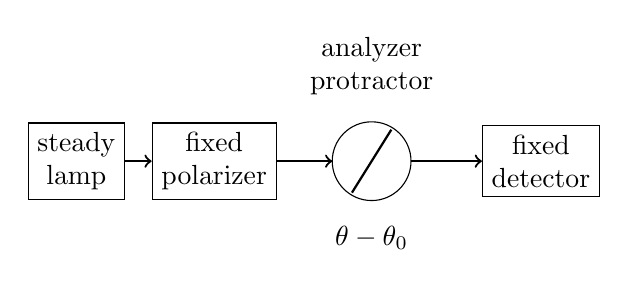
\begin{tikzpicture}[x=1cm,y=1cm]
 \node[draw,align=center] (s) at (.6,0) {steady\\lamp};
 \node[draw,align=center] (p) at (2.35,0) {fixed\\polarizer};
 \draw (4.35,0) circle (.5);\draw[thick] (4.1,-.4)--(4.6,.4);
 \node[above,align=center] at (4.35,.72) {analyzer\\protractor};
 \node[draw,align=center] (d) at (6.5,0) {fixed\\detector};
 \draw[->,thick] (s)--(p);\draw[->,thick] (p.east)--(3.85,0);
 \draw[->,thick] (4.85,0)--(d.west);\node[below] at (4.35,-.7) {$\theta-\theta_0$};
\end{tikzpicture}
\caption{Fixed illumination and detector geometry with a rotating analyzer. The protractor angle is observed only after the light has settled.}
\label{fig:malus-law-apparatus}
\end{figure}

The data contain ten states from $0$ to $90$ degrees in $10$-degree increments, each lasting approximately six seconds. A paired observation includes the manual angle, one light count and its device and receive times. The captured count and both times match the continuous light record, so the snapshot association can be checked without assuming that the two clocks are equal.

For each setting $j=0,\ldots,9$, we also compute a mean over $[6j+1,6j+5.5)\unit{s}$ on the device clock. These 4.5-second interior windows exclude rotations and state boundaries. The resulting two reductions---one count per accepted observation and one mean per settled state---share the same ten angle values. They must not be interpreted as independent experiments.

\section{A fit that keeps angle zero explicit}
The example's specified normalization is $(S-10)/1000$, equivalent to a floor of 10 counts and a parallel signal of 1010 counts. At zero degrees, the snapshot is 1029 counts, giving normalized transmission 1.019. At ten degrees, it is 1020 counts, giving 1.010 even though the ideal cosine-squared value is 0.96985. A value above unity is a useful diagnostic of the specified reference, rather than a reason to truncate the observation.

To estimate the shape without fixing the floor or parallel signal, rewrite Eq.~\eqref{eq:malus-law-model} as
\begin{equation}
 S=a+b\cos2\theta+c\sin2\theta.
 \label{eq:malus-law-harmonic}
\end{equation}
An unweighted linear least-squares solution gives $A=2\sqrt{b^2+c^2}$, $B=a-\sqrt{b^2+c^2}$ and $\theta_0=\tfrac12\operatorname{atan2}(c,b)$. The trigonometric arguments use radians internally. This parameterization handles an angular-zero offset without a logarithm near extinction, where both the signal and a cosine can approach zero.

\begin{figure}[!htbp]
\centering% Generated by prepare_drafts.py from the supplied CSV files.
\begin{tikzpicture}
\begin{groupplot}[group style={group size=1 by 2,vertical sep=1.15cm},
width=0.98\columnwidth,height=3.2cm,
grid=major,enlarge x limits=false,
legend style={font=\scriptsize,at={(0.5,1.03)},anchor=south,
legend columns=4,draw=none,fill=none,column sep=4pt},
title style={font=\scriptsize,at={(0.02,0.98)},anchor=north west,
fill=white,fill opacity=0.9,text opacity=1,inner sep=2pt},
ylabel style={font=\footnotesize},
xlabel style={font=\footnotesize},tick label style={font=\scriptsize}]
\nextgroupplot[ylabel={Transmission (1)},width=0.96\columnwidth,enlarge x limits=0.03,ymin=-0.05,ymax=1.3,title={(a) Polarization response}]
\addplot[csblue,solid,line width=0.8pt,only marks,mark=*] table[col sep=comma,x=c0,y expr={(\thisrow{c1}-(0))*(1)}] {data/drafts/optics-malus-observations.csv};
\addlegendentry{Snapshot}
\addplot[csred,dashed,line width=0.8pt] table[col sep=comma,x=c0,y expr={(\thisrow{c1}-(0))*(1)}] {data/drafts/optics-malus-fit.csv};
\addlegendentry{Mean fit}
\nextgroupplot[ylabel={Residual (1)},width=0.96\columnwidth,enlarge x limits=0.03,ymin=-0.003,ymax=0.055,xlabel={Analyzer angle (degree)},title={(b) Relative to $\cos^2\theta$}]
\addplot[csblue,solid,line width=0.8pt,only marks,mark=*] table[col sep=comma,x=c0,y expr={(\thisrow{c4}-(0))*(1)}] {data/drafts/optics-malus-observations.csv};
\addlegendentry{Snapshot}
\addplot[csteal,dashdotted,line width=0.8pt,only marks,mark=triangle*] table[col sep=comma,x=c0,y expr={(\thisrow{c5}-(0))*(1)}] {data/drafts/optics-malus-observations.csv};
\addlegendentry{4.5-s mean}
\end{groupplot}
\end{tikzpicture}

\caption{Upper: snapshot transmission and harmonic fit to settled means. Lower: snapshot and settled-mean residuals relative to $\cos^2\theta$, with the specified normalization retained. Their positive offset identifies the reference mismatch.}
\label{fig:malus-law-example}
\end{figure}

\begin{table}[!htbp]
\caption{Harmonic-fit parameters for snapshots and 4.5-s means. Residual RMS summarizes scatter about each fit.}
\label{tab:malus-law-values}
\centering\footnotesize
\begin{tabular}{@{}lrr@{}}\toprule
Quantity & Snapshots & 4.5-s means\\\midrule
$A$ (counts) & 1024.56 & 1020.44\\
$B$ (counts) & 13.20 & 13.04\\
$\theta_0$ (degrees) & $-0.097$ & 0.012\\
Residual RMS (counts) & 7.13 & 0.51\\\bottomrule
\end{tabular}
\end{table}

The plateau fit implies a parallel response near 1033.5 counts, explaining the predominantly positive residuals against the specified 1010-count reference. The snapshot residual RMS relative to the fixed unit-amplitude, zero-offset cosine-squared curve is 0.0186 in normalized signal. Allowing amplitude, floor and zero to vary separates the fitted optical response from scatter around the model.

Averaging substantially reduces residual scatter. The fitted angular zero is a point estimate whose uncertainty depends on the protractor resolution and angular calibration. Reporting the numerical phase to hundredths of a degree distinguishes the fit's numerical precision from the uncertainty of the angle reference.

\section{Identifiability near extinction}
The fitted floor combines every contribution that is approximately independent of angle: detector offset, ambient light, incomplete polarization and analyzer leakage can all enter $B$. A single sweep cannot identify these separately. A covered-detector reading, a source-off reading and a crossed-analyzer reading are physically different observations and should be compared before attributing the floor to polarizer extinction.

The angular sensitivity of normalized ideal transmission is $dT/d\theta=-\sin2(\theta-\theta_0)$ when angle is expressed in radians. Near 45 degrees, a one-degree zero error changes transmission by approximately 0.0175. Near parallel and crossed settings, the first derivative vanishes, so the same error enters at higher order. A small residual at the extrema is therefore a weak test of angular calibration; intermediate angles carry much of that information.

The example sequence supports a cosine-squared angular dependence after explicit allowance for its scale and floor. Repeating the sweep in both directions would distinguish backlash or angle-reading hysteresis from a stationary optical response. Rotating only the analyzer, retaining a stable spectrum and independently characterizing the floor are more informative than increasing the displayed fit precision.
